\documentclass[a4paper,12pt]{article}

\usepackage{mathtext}
\usepackage[T2A]{fontenc}
\usepackage[utf8]{inputenc}
\usepackage[russian]{babel}
\usepackage{multirow}
\usepackage{slashbox}
\usepackage{makecell}
\usepackage{graphicx}
\usepackage{physics}
\usepackage{amstext}
\usepackage{caption}
\usepackage{subcaption}
\usepackage{cmap}
\usepackage{float}


\title{Лабораторная работа 7}
\author{Калашников Михаил, Б03-205}
\date{}

\begin{document}

\maketitle{Время, которого мало}

\begin{enumerate}

\setcounter{enumi}{0}

\item Напишем страшненький цикл, каждая итерация которого будет содержать много последовательных операций сложения. Измерим время и получим следующие результаты:

\begin{figure}[H]
  \centering
  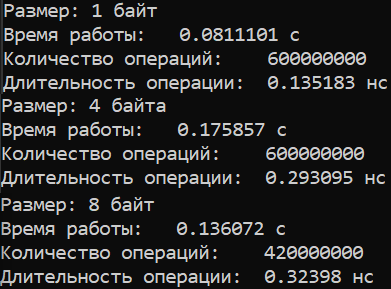
\includegraphics[width=1\linewidth]{images/asm7_1.png}
\end{figure}

\item Будем обходить матрицу. Как можно заметить, обход по строкам значительно быстрее обхода по столбцам.

\begin{figure}[H]
  \centering
  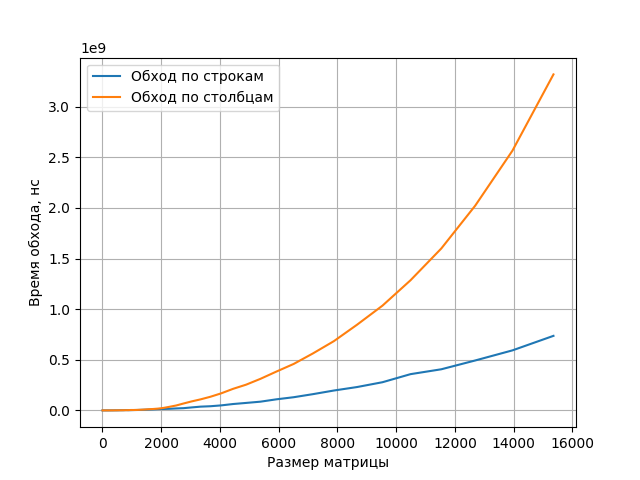
\includegraphics[width=1\linewidth]{images/asm7_2.png}
\end{figure}

\item Теперь будем обходить одномерный массив интов по заранее сгенерированным случайным индексам. Построим график и заметим резкий скачок. Он происходит когда размер массива начинает превышать размер кэша процессора. 

\begin{figure}[H]
  \centering
  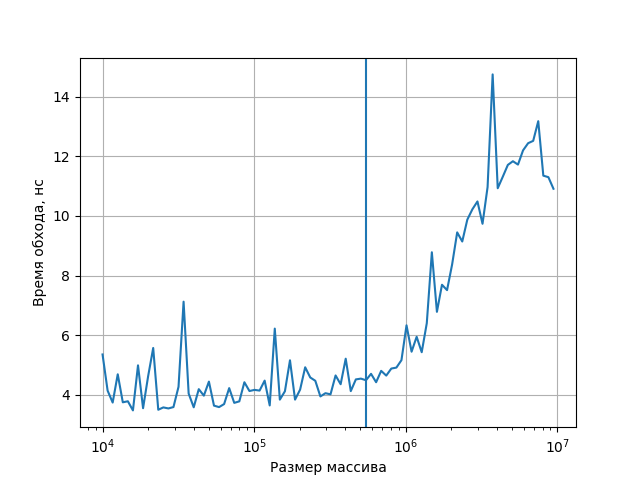
\includegraphics[width=1\linewidth]{images/asm7_3.png}
\end{figure}

\item Скачок происходит приблизительно при размере массива, равном $5.5\cdot10^5$. Это соответствует 2.1 мегабайтам памяти. Согласно диспетчеру задач один из кэшей моего процессора (L2) равен 2 мегабайтам.

\item Со списком такой эффект повторить тяжелее, потому что описанные операции занимают значительно больше времени (и вообще не предусмотрены для списка!). Но я смог заметить незначительное изменение, отраженное на графике.

\begin{figure}[H]
  \centering
  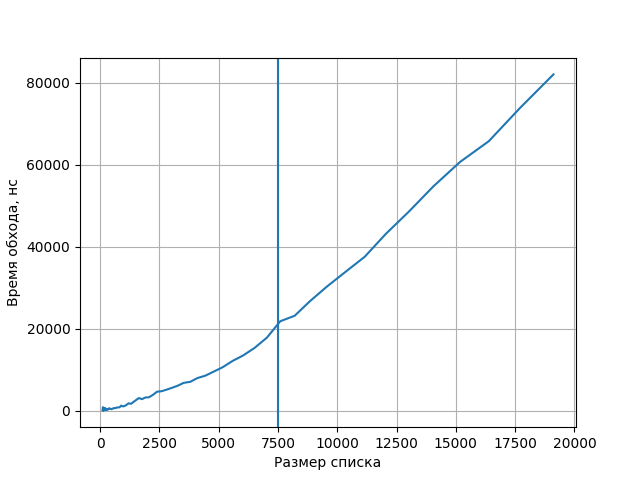
\includegraphics[width=1\linewidth]{images/asm7_4.png}
\end{figure}

\item Выделение новой памяти с помощью new занимает примерно 20-23 нс. malloc занимает столько же времени. delete требует 10-12 нс, а free -- 9-10 нс.

Вот пример кода, измеряющего время delete.

\begin{figure}[H]
  \centering
  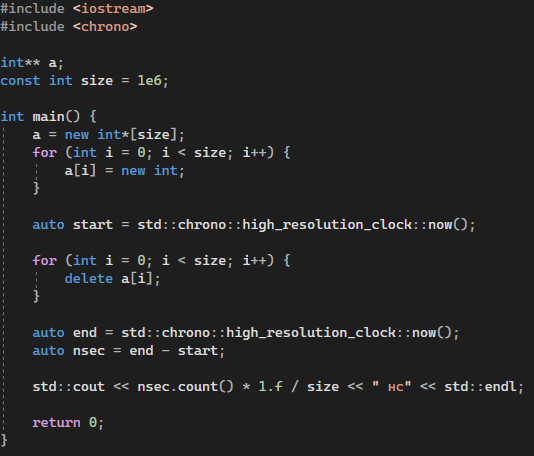
\includegraphics[width=1\linewidth]{images/asm7_5.png}
\end{figure}

\item shared\_ptr и unique\_ptr создаются в среднем за 140 нс, а  за 65 нс.

\item Разыменование указателей (обычных и умных) происходит быстро, примерно за 3-3.5 нс.

Вот так я измерял это время (в листинге убрал прибавление 23)

\begin{figure}[H]
  \centering
  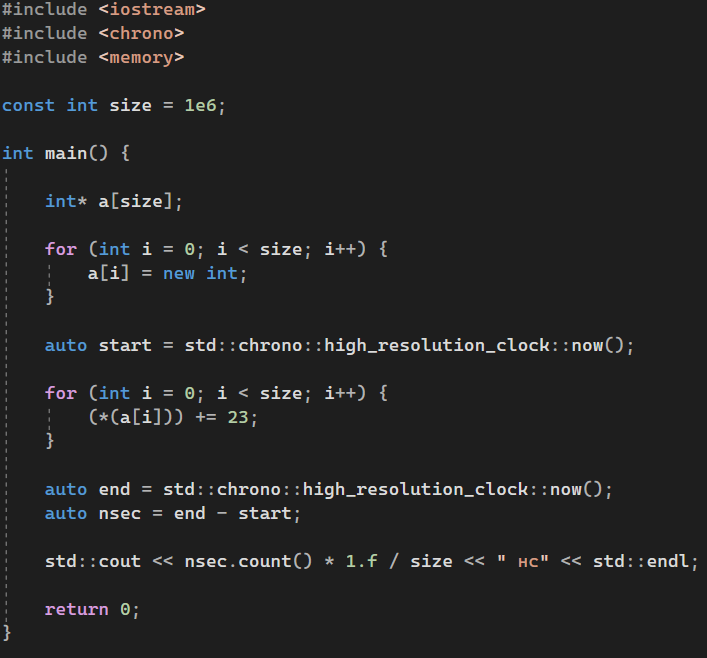
\includegraphics[width=1\linewidth]{images/asm7_6.png}
\end{figure}


\end{enumerate}

\end{document}